\section{\lang{Introduction}{Introducción}}

\ifthenelse{\equal{\LANG}{es}}{
      En los últimos años ha habido muchas mejoras en el campo de aprendizaje por refuerzo. Con nuevos diseños de arquitecturas y grafos de recompensa se han superado a jugadores profesionales en juegos como el Go~\cite{silver2016go} o el StarCraft II~\cite{vinyals2019starcraft}. Sin embargo, el campo de aprendizaje por refuerzo es todavía un campo abierto por explorar, especialmente en su aplicación a entornos de alta complejidad.
}{}
\ifthenelse{\equal{\LANG}{en}}{
      In recent years, reinforcement learning has achieved remarkable progress. Advances in neural architectures and reward design have enabled agents to outperform professional players in highly complex games such as Go~\cite{silver2016go} and StarCraft II~\cite{vinyals2019starcraft}. Nevertheless, reinforcement learning remains a developing field, particularly in domains that involve intricate and uncertain environments.
}{}

\ifthenelse{\equal{\LANG}{es}}{
      Pokémon es una franquicia de videojuegos que se ha extendido a otros medios como el anime, el manga o los juegos de cartas. Tiene varios juegos competitivos (Unite, GO, TCG), pero en el que se centra este TFG es en las batallas de los juegos principales.
}{}
\ifthenelse{\equal{\LANG}{en}}{
      Pokémon is a video game franchise that has expanded into multiple forms of media, including anime, manga, and trading card games. Although the franchise features several competitive titles, such as Unite, GO, and the Trading Card Game (TCG), this Thesis focuses on battles in the mainline games.
}{}

\ifthenelse{\equal{\LANG}{es}}{
      Dentro de los juegos principales, hay distintos formatos de batalla. Cada uno tiene sus propias reglas y restricciones: qué Pokémon y movimientos están disponibles, el número de jugadores, si se requiere elegir un equipo de antemano o no, el número de Pokémon que se controlan en el campo, etc. Todos estos formatos se caracterizan por ser juegos de suma cero con un elevadísimo número de estados, información oculta, actuación simultánea y un alto grado de estocasticidad. El formato en el que se centra este TFG es el de batallas aleatorias individuales de la generación IX \emph{gen9randombattle}, cuya característica principal es que el simulador genera un equipo aleatorio por jugador.
}{}
\ifthenelse{\equal{\LANG}{en}}{
      The mainline games offer a variety of battle formats, each defined by its own set of rules and restrictions, including the available Pokémon and moves, the number of players, whether teams are selected in advance, and the number of Pokémon active on the battlefield. Despite these differences, all formats share several characteristics: they are zero-sum games with enormous state spaces, hidden information, simultaneous decision-making, and a high degree of stochasticity. This Bachelor's Thesis focuses on the Generation IX Random Battle Singles format (\emph{gen9randombattle}), in which the simulator generates a random team for each player at the start of every battle.
}{}

\ifthenelse{\equal{\LANG}{es}}{
      Tal como se puede ver en la figura \ref{fig:CombatePokemon}, los combates Pokémon de la generación IX se desarrollan por turnos entre dos entrenadores, cada uno de los cuales dispone de un equipo de hasta seis Pokémon. En cada turno, los jugadores deben elegir una acción para su Pokémon activo, como utilizar uno de los movimientos disponibles o realizar un cambio de Pokémon. Una vez seleccionadas las acciones, estas se ejecutan siguiendo un orden determinado principalmente por la estadística de Velocidad de los Pokémon involucrados, aunque puede haber otros condicionantes que alteren dicho orden. El resultado de cada acción depende de diversos factores, entre los que se encuentran las estadísticas de combate de los Pokémon, la potencia y el tipo de los movimientos utilizados, las interacciones entre tipos y determinados efectos de estado o de campo. El combate concluye cuando todos los Pokémon de uno de los entrenadores han sido debilitados. Además, la novena generación incorpora la mecánica de la \textit{Teracristalización}, que permite modificar el tipo de un Pokémon durante el combate, introduciendo nuevas posibilidades estratégicas tanto en ataque como en defensa.
}{}
\ifthenelse{\equal{\LANG}{en}}{
      As illustrated in Figure \ref{fig:CombatePokemon}, Generation IX Pokémon battles take place in a turn-based setting between two trainers, each controlling a team of up to six Pokémon. At every turn, both players simultaneously choose an action for their active Pokémon, such as using one of its available moves or switching to another team member. Once the actions have been selected, they are executed according to an order determined primarily by the Pokémon's Speed stat, although other factors may alter this priority. The outcome of each action depends on multiple factors, including the Pokémon's battle stats, the power and type of the selected moves, type interactions, and various status or field effects. A battle ends when all the Pokémon on one trainer's team have fainted. In addition, Generation IX introduces the \textit{Terastallization} mechanic, which allows a Pokémon to temporarily change its type during battle, creating new strategic opportunities in both offensive and defensive play.
}{}


\begin{figure}[t]
      \centering
      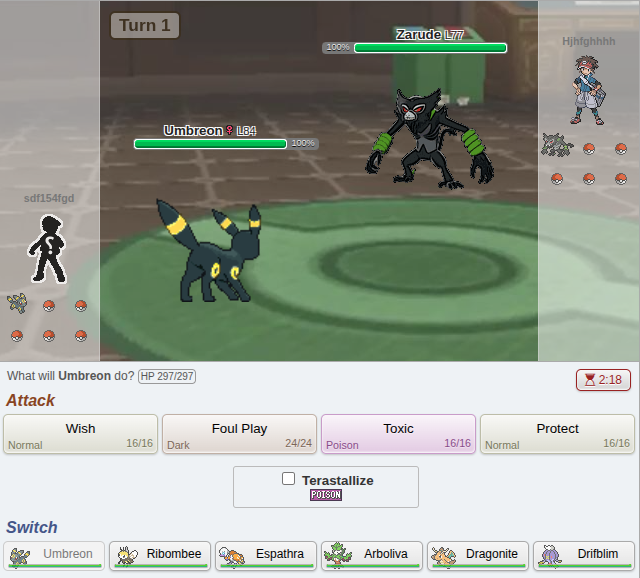
\includegraphics[width=0.7\textwidth]{images/CombatePokemon.png}
      \caption[\lang{Example of a \emph{gen9randombattle} Pokémon battle}{Ejemplo de combate Pokémon \emph{gen9randombattle}}]{\lang{{Example of a \emph{gen9randombattle} Pokémon battle. The player's six Pokémon are shown at the bottom of the figure, whereas the opponent's Pokémon remain hidden until they are sent into battle.}}{Ejemplo de combate Pokémon \emph{gen9randombattle}. Se pueden observar los seis Pokémon propios en la parte inferior de la figura, mientras que los Pokémon del otro jugador están ocultos hasta el turno en que se usan en combate.}}
      \label{fig:CombatePokemon}
\end{figure}


\ifthenelse{\equal{\LANG}{es}}{
      \textbf{Contribución del TFG:} como Pokémon todavía es un problema abierto en el campo de aprendizaje por refuerzo, este trabajo propone un nuevo enfoque multiagente aplicado a las batallas aleatorias individuales de la generación IX disponibles en la plataforma Pokémon Showdown~\cite{pokemonShowdown}. El simulador existente no permite repetir batallas ni comenzar desde un punto intermedio, lo cual constituye un desafío adicional. Este problema representa una considerable dificultad de investigación, por lo que se explorarán diferentes técnicas de aprendizaje multiagente y estrategias de \textit{reward shaping}.
}{}
\ifthenelse{\equal{\LANG}{en}}{
      \textbf{Thesis contribution:} since Pokémon battles remain an open challenge for reinforcement learning, this Thesis proposes a novel multi-agent reinforcement learning approach for the Generation IX Random Battle Singles format available on Pokémon Showdown~\cite{pokemonShowdown}. Furthermore, the simulator imposes additional constraints, as battles cannot be replayed or resumed from intermediate states. This limitation presents a significant research challenge, motivating the exploration of various multi-agent learning techniques and \textit{reward shaping} strategies.
}{}

\ifthenelse{\equal{\LANG}{es}}{
      Para entrenar el modelo se usarán distintas técnicas como Actor-Critic y grafos de recompensa complejos para encontrar un modelo y método de entrenamiento que funcione de manera eficiente.
}{}
\ifthenelse{\equal{\LANG}{en}}{
      To train the model, various techniques such as Actor-Critic methods and complex reward graphs will be employed to identify an effective model and training procedure.
}{}

\ifthenelse{\equal{\LANG}{es}}{
      El estudio del aprendizaje por refuerzo en entornos lúdicos como las partidas de Pokémon no solo tiene interés desde el punto de vista recreativo o experimental, sino que también puede aportar conocimientos transferibles a otros dominios. Los videojuegos en general son entornos complejos y dinámicos que permiten evaluar el comportamiento de los agentes en situaciones de decisión secuencial bajo incertidumbre. Las técnicas desarrolladas y validadas en estos contextos pueden generalizarse posteriormente a problemas como la optimización de procesos industriales, la toma de decisiones en sistemas financieros, la planificación logística o el control de sistemas autónomos.
}{}
\ifthenelse{\equal{\LANG}{en}}{
      Studying reinforcement learning in gaming environments such as Pokémon battles is valuable not only from a recreational or experimental perspective, but also because of its potential applicability to real-world problems. Video games provide complex, dynamic, and highly stochastic environments in which intelligent agents can be evaluated on sequential decision-making tasks under uncertainty. Techniques developed and validated in these settings may later be transferred to practical applications, including industrial process optimization, logistics planning, decision-making in financial systems, and the control of autonomous systems.
}{}
